\documentclass[a4paper]{article}

\usepackage[english]{babel}
\usepackage[utf8]{inputenc}
\usepackage{amsmath}
\usepackage{graphicx}
\usepackage[colorinlistoftodos]{todonotes}


\title{Numerical Simulation: Assignment 2}

\author{Sjoerd Hooijmaaijers - ANR: 496687}

\date{\today}

\begin{document}
\maketitle



\section{Introduction}

For this assignment, I have chosen to pick previous assignments from the course Generational Economics.
Fearing that only one may have been too short, I will include the first and the second (out of a total of 6) assignment of this course.
Both have mathematical derivations, but perhaps lack a few words.

\section{Generational Economics Assignment 1}
Assume that production is described by $Y=AK^a L^b$, A, a and b are positive constants
\subsection{Question 1}
\subsubsection*{ i. Is this production function neoclassical? Which of the neoclassical conditions does it satisfy and which ones not?}
There are three conditions for a neoclassical function.\\
Condition 1: Constant returns to scale \\
$ \lambda Y = F(\lambda K,\lambda L)$ \\
$ \lambda Y = A*\lambda K^a*\lambda L^b$ \\
$ \lambda Y = A*\lambda ^{a+b}* K^a* L^b$ \\
$ \lambda Y = \lambda ^{a+b}F(\lambda K,\lambda L)$ \\

Thus, a+b=1 \\ 
And similarly; b=1-a \\
Since a and b are positive constants, we know that: 

\begin{itemize}
\item $0<a<1$
\item $0<b<1$
\end{itemize} 

Condition 2: Positive but diminishing returns

$$ \frac{\delta F}{\delta K} = aAK^{a-1}L^{1-a} > 0 $$ \\
$$ \frac{\delta ^2 F}{\delta K^2} = (a-1)aAK^{a-2}L^{1-a} < 0		$$ \\
$$ \frac{\delta F}{\delta L} = aAK^{a}L^{-a} > 0 $$ \\
$$ \frac{\delta ^2 F}{\delta L^2} = -a(1-a)AK^{a}L^{-a-1} < 0		$$ \\

Condition 3. Inada conditions \\
The marginal product of capital is \\
$$ MPK = aAK^{a-1}L^{1-a} $$ \\
$$ = aA\frac{K}{L}^{a-1} $$ \\
and thus
$$ \lim_{k\to\infty} aA \frac{K}{L}^{a-1} =0 $$ \\
$$ \lim_{k\to 0} aA \frac{K}{L}^{a-1} = \infty $$ \\
\\
The marginal product of labour is \\
$$ MPL = (1-a)AK^{a}L^{-a} $$ \\
$$ = (1-a)A\frac{K}{L}^{a} $$ \\
and thus
$$ \lim_{k\to\infty} (1-a)A \frac{K}{L}^{a} =0 $$ \\
$$ \lim_{k\to 0} (1-a)A \frac{K}{L}^{a} = \infty $$ \\

In conclusion, all three requirements are fulfilled

\subsubsection*{ii. Write output per labour efficiency unit (y) as a function of capital per labour
efficiency unit (k). What is the marginal product of k?}

Remember we can write the production function as \\
$$ Y=AK^a L^{a-1} $$ \\
Then, taking per labour efficiency units \\
$$ \frac{Y}{L}= A \frac{K}{L}^{a} \frac{L}{L}^{a-1} $$ \\
Or in other terms \\
$$ y=Ak^a $$ \\

Then the marginal product of k is: \\
$$ f(k)=Ak^a $$ \\
$$ f'(k)=aAk^{a-1} $$ \\

\subsubsection*{iii. Assume that an economy is in a dynamically inefficient steady state when the rate of population growth n rises to a permanently higher level. Assume that investment per labour efficiency unit i does not change and that the capital-labour ratio converges to a new steady-state level. Will utility in the long run increase or decrease? Explain your answer!}

Taking that the economy starts off in a dynamically inefficient steady-state, it is located somewhere in the right hand side of the above graph. \\ If the rate of population growth increases, and holding investment per labor efficiency unit constant, we can state, from the equation in $i=(\delta+g)k$, that capital-labor ratio will decrease (intuitively, it makes sense considering that population now grows quicker – and so will labor – while, for capital, we see no difference); graphically, this means that the steady-state will now be represented further to the left. \\Given this, in the long-run, utility will increase as consumption increases, as the economy approaches its optimal capital-labor ratio. \\
However, it is important to denote that if the decrease in k is large enough, it could also lead to the Golden Rule capital-labor ratio being surpassed, which would lead to a less-than-optimal utility. \\
\begin{figure}
  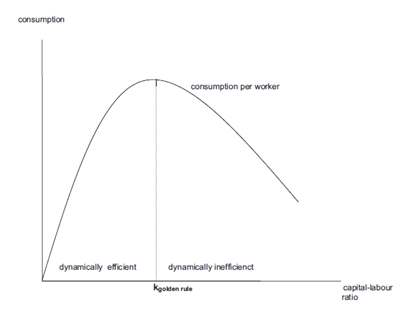
\includegraphics[width=\linewidth]{Ass2.png}
 

\end{figure}



\end{document}